\chapter{Computer vision}
With the rise of the Internet and modern technologies, we can now confirm with certainty that we live in an image-based society, the video sharing platform Youtube is responsible for 37\% of all mobile internet traffic alone (see Figure ~\ref{fig:youtube}).

\begin{figure}[H]
  \centering
  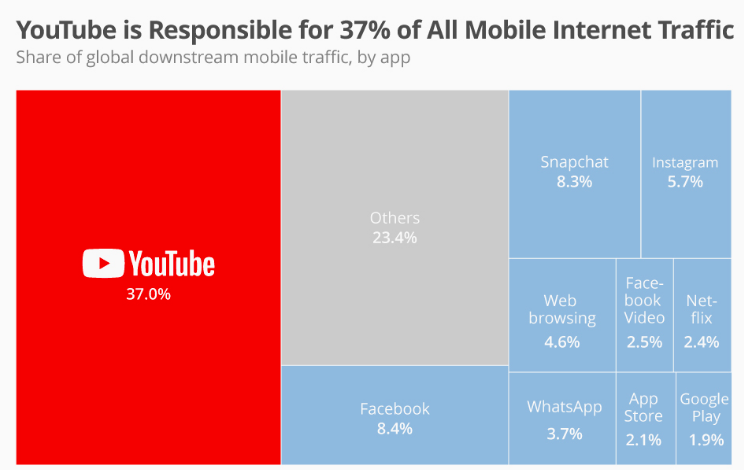
\includegraphics[width=.8\linewidth]{youtube_traffic.png}
  \caption{Youtube internet traffic share. \href{https://www.statista.com/chart/17321/global-downstream-mobile-traffic-by-app}{Source}}
  \label{fig:youtube}
\end{figure}

With about 3.5 billion smartphone users\cite{stats_smartphone_usage}, a huge part using massively visual content sharing platforms, the amount of information transmitted by this data is enormous, so automating the abstract information extraction of these pixels has an unimaginable potential.
Computer Vision is a technology that allows computers to extract abstract information from visual content.

\pagebreak\section{What is it}
The term "computer vision" refers to the different techniques that allow computers to see and understand the content of images. This is a sub-category of artificial intelligence and machine learning.

The computer vision field brings together multiple techniques from various fields of engineering or computer science. In general, the different methods aim to reproduce the human vision. To understand the content of images, machines must be able to extract a description: an object, a description, a 3D model...

Some computer vision systems may also require image processing, i.e. simplifying or augmenting the content of the image. Examples include normalizing the photo-metric properties of the image, cropping its contours or removing noise such as digital artifacts induced by low light.

\pagebreak\section{Challenges}

What could be simpler than vision? From birth, humans are naturally able to see. However, allowing a computer to do the same is not an easy task. To date, computer vision still fails to match human vision.

One of the reasons is that we still do not really know how human vision works. We need to understand how perceptual organs such as the eyes work, but also how the brain interprets this perception. Although research in this area is progressing at a rapid pace, we are still a long way from unlocking all the mysteries of vision.

Another challenge is related to the complexity of the visual world. An object can be perceived from multiple angles, under various lighting conditions, partial hidden by other objects...

A true computer vision system must be able to perceive the content in any of these situations and extract information from it. In fact, computer vision is a real scientific challenge.

\pagebreak\section{Deep learning}

Several years ago, most computer vision algorithms consisted of simple heuristics to extract features from pixels (See an example of heuristic on Figure ~\ref{fig:haar}).
\begin{figure}[H]
  \centering
  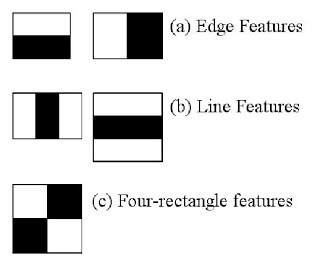
\includegraphics[width=.35\linewidth]{haar_classifier.jpg}
  \caption{Haar features. \href{https://towardsdatascience.com/learning-computer-vision-41398ad9941f}{Source}}
  \label{fig:haar}
\end{figure}
Over time, there has been more and more use of machine learning and such automatic pattern recognition algorithm, the true revolutionising technology that have made machine learning in general works so well is neural networks and especially deep neural networks (see Figure ~\ref{fig:deeplearning}).

\begin{figure}[H]
  \centering
  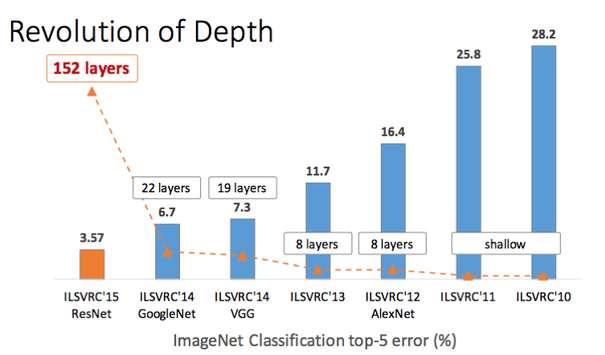
\includegraphics[width=.7\linewidth]{deep_learning.png}
  \caption{Revolution of depth, from a few network layers to hundred(s). \href{https://towardsdatascience.com/learning-computer-vision-41398ad9941f}{Source}}
  \label{fig:deeplearning}
\end{figure}
\pagebreak
In addition to deep neural networks, we saw a birth of a game breaking algorithm in computer vision, it has been called "convolutional" neural network (CNN)\cite{originalcnn}.
The difference with CNN and dense network is that CNN take advantage of the hierarchical pattern in images (see Figure ~\ref{fig:cnn}).

\begin{figure}[H]
  \centering
  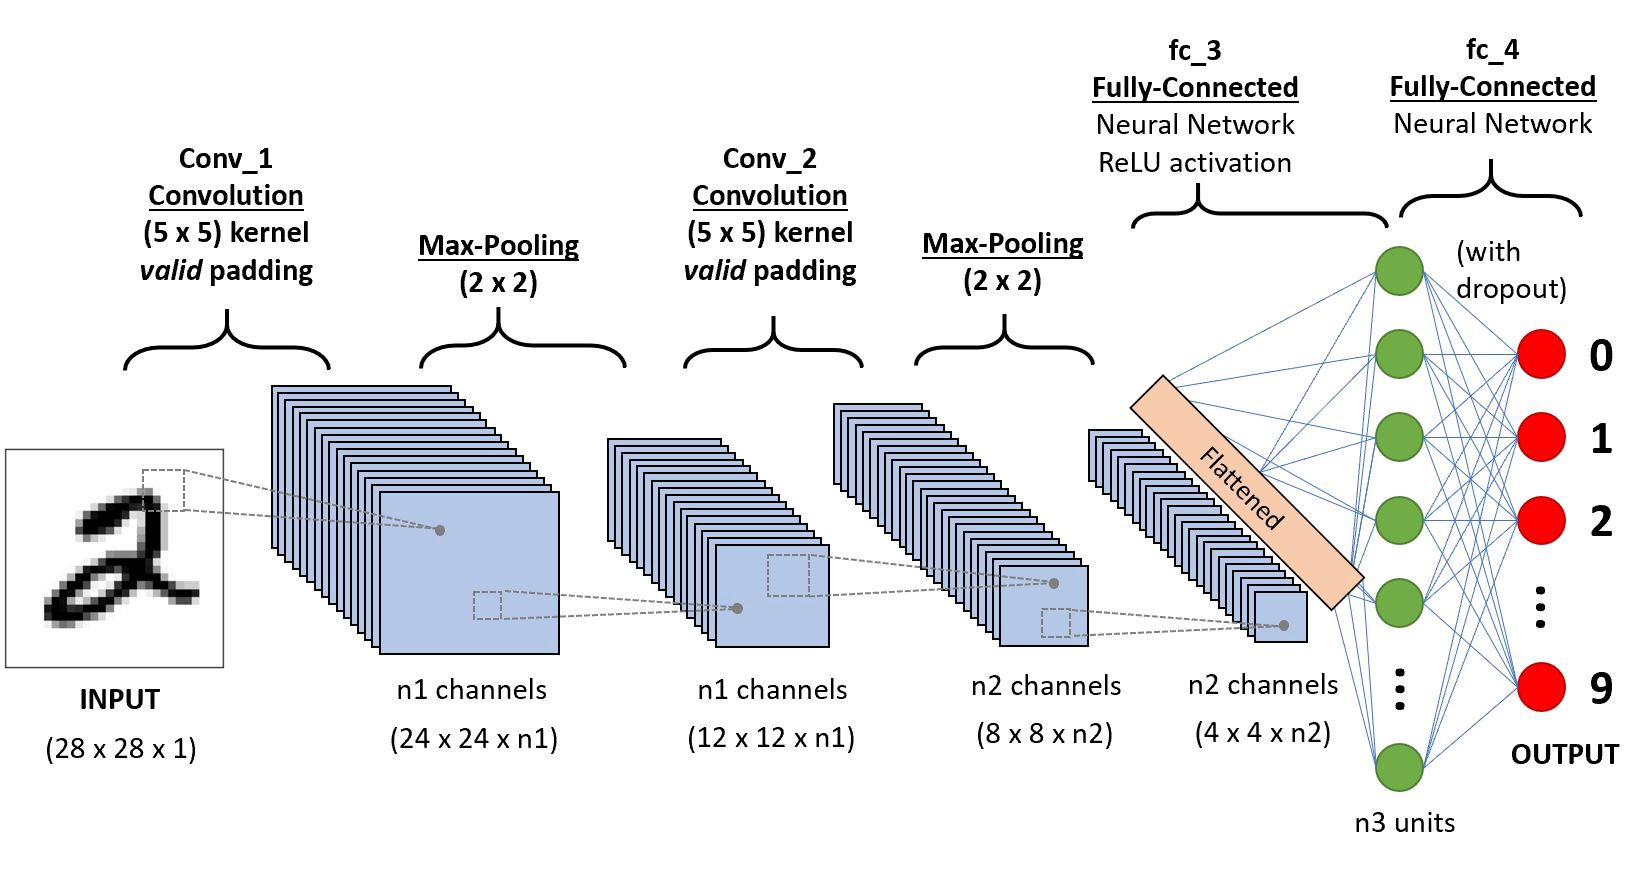
\includegraphics[width=0.9\linewidth]{cnn.jpeg}
  \caption{Convolutional neural network. \href{https://towardsdatascience.com/a-comprehensive-guide-to-convolutional-neural-networks-the-eli5-way-3bd2b1164a53}{Source}}
  \label{fig:cnn}
\end{figure}

\pagebreak\section{Applications}

Despite the difficulties associated with the development of computer vision, the considerable advances made over the years have already enabled Computer Vision to perform many tasks.

This technology is proving to be effective for optical character recognition, also known as "OCR", everyone with an Android smartphone can use it through Google Lens (see Figure ~\ref{fig:glens}).
\begin{figure}[H]
  \centering
  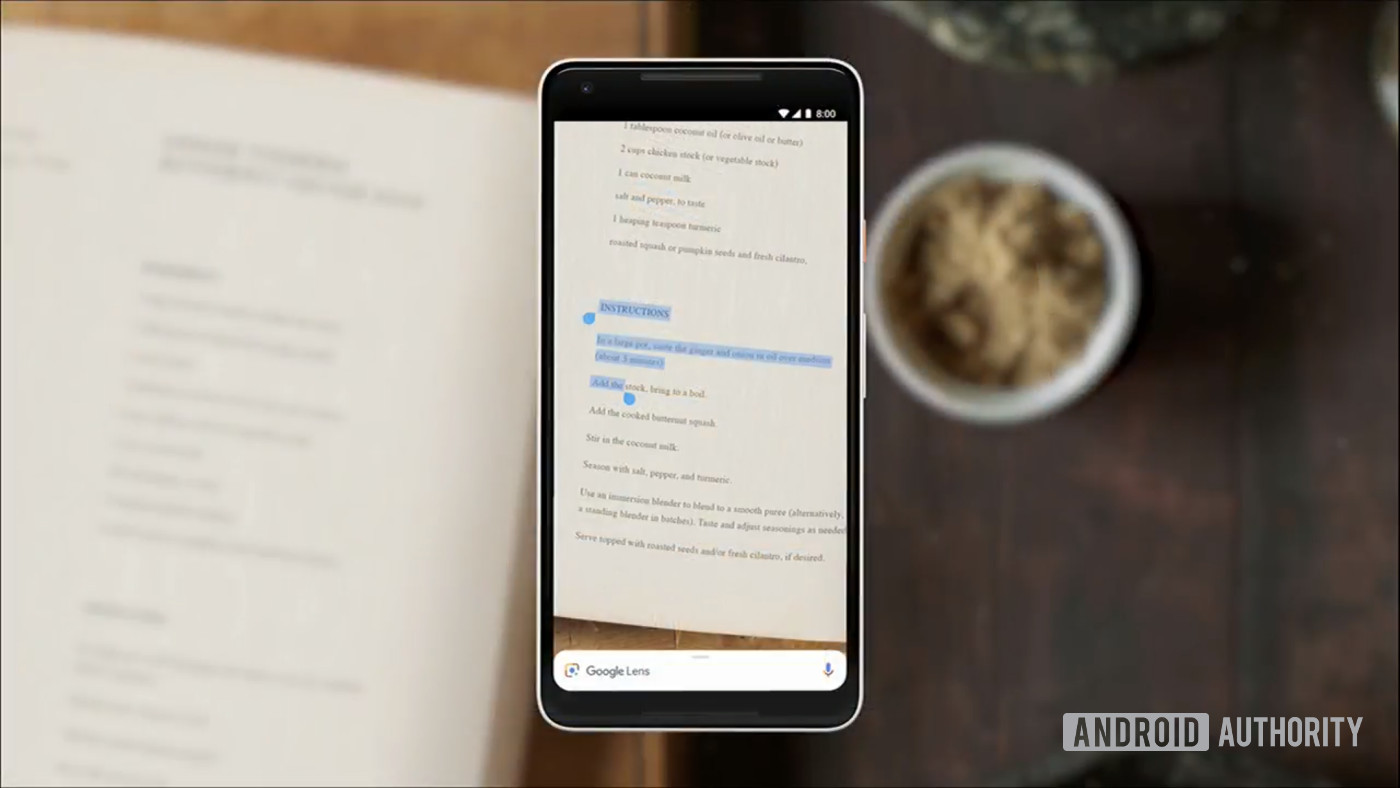
\includegraphics[width=.8\linewidth]{google-lens-smart-text-selection.jpg}
  \caption{Optical character recognition directly on your smartphone with Google Lens. \href{https://www.androidauthority.com/google-lens-camera-app-863117/}{Source}}
  \label{fig:glens}
\end{figure}
\pagebreak
In the field of automotive safety, computer vision is used for hazard detection. With the emergence of autonomous cars, computer vision will soon occupy a central place in the automotive industry as it will allow vehicles to see on the road (see an example of image segmentation in the field of smart vehicles on Figure ~\ref{fig:carseg}).

\begin{figure}[H]
  \centering
  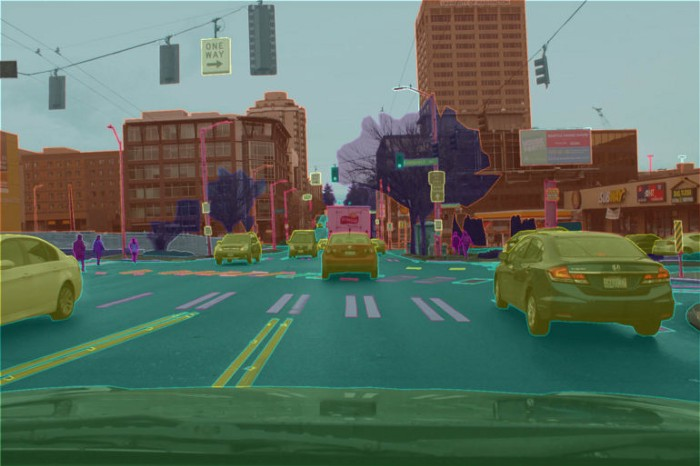
\includegraphics[width=.8\linewidth]{image_segmentation.jpg}
  \caption{Image segmentation on the road. \href{https://towardsdatascience.com/learning-computer-vision-41398ad9941f}{Source}}
  \label{fig:carseg}
\end{figure}%

\pagebreak
It is also used in the film industry for "match move", i.e. to synchronize computer-generated images with the real actors. It is also used for motion capture.

The facial recognition technologies of the latest smartphones, such as the famous Face ID of Apple's latest iPhone, are also based on Computer Vision. The same technology is used by automatic surveillance cameras (see face-related applications on Figure ~\ref{fig:facreco}).
\begin{figure}[H]
\centering
\begin{subfigure}{.5\textwidth}
  \centering
  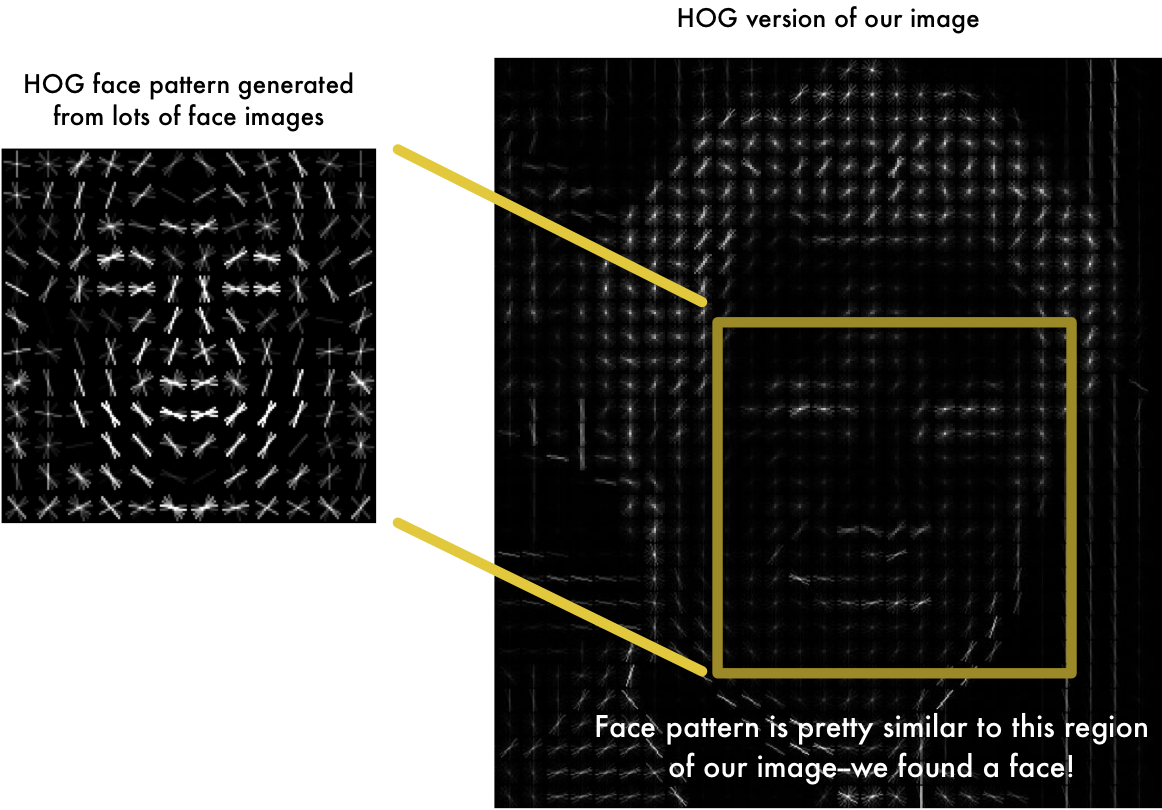
\includegraphics[width=.8\linewidth]{hog.png}
  \caption{Histogram of oriented gradients (used in facial recognition) \href{https://medium.com/@ageitgey/machine-learning-is-fun-part-4-modern-face-recognition-with-deep-learning-c3cffc121d78}{Source}}
\end{subfigure}%
\begin{subfigure}{.5\textwidth}
  \centering
  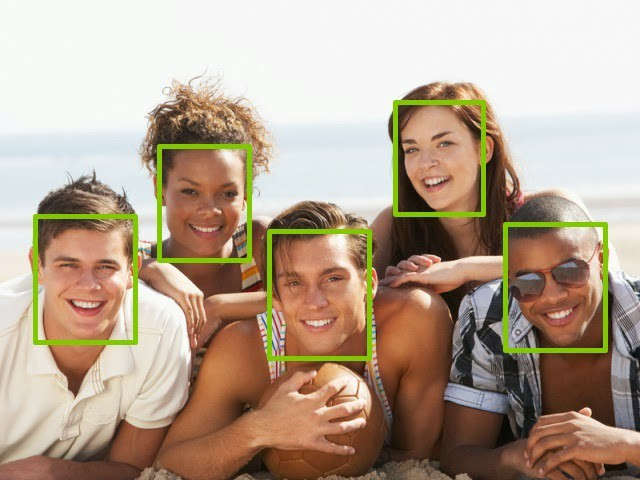
\includegraphics[width=.8\linewidth]{face_detection.jpg}
  \caption{Face detection. \href{https://towardsdatascience.com/learning-computer-vision-41398ad9941f}{Source}}
\end{subfigure}
\caption{Examples of face-related applications}
\label{fig:facreco}
\end{figure}

As you will have understood, computer vision is used in a wide range of fields. As this technology develops, the opportunities it offers will increase in the coming years. Soon, all machines will probably be able to see, in exactly the same way as human beings and better ...

Computer vision is not yet very practical to use on our current everyday interfaces: smartphones.
In the future, we can imagine increasing human vision by coupling it with computer vision via mixed reality glasses, for example looking at a monument, having its history displayed on the glasses...